\section{The State-of-the-Art}
\label{sec:state-of-the-art}

This leads us to the current state-of-the-art approach for compressing nanopore
signal data which we will appropriately name zstd-svb-zd, although VBZ is the
name ONT uses to describe it \cite{vbz}.

%VBZ16 is equivalent to VBZ \cite{vbz} but Stream VByte is replaced with Stream VByte 16.

zstd-svb-zd consists of the following encodings applied successively:
\begin{enumerate}
\item differential coding,
\item zig-zag encoding,
\item svb and
\item zstd.
\end{enumerate}

Differential coding is a bijective function from $\mathbb{R}^n\to\mathbb{R}^n$ classically defined as
\[ (x_1, x_2, \dots, x_n) \mapsto (\delta_1,\delta_2,\dots,\delta_n) = (x_1, x_2 - x_1, x_3-x_2,\dots,x_n-x_{n-1}). \]
That is, the original data is replaced by the differences (or \textit{deltas}) between successive data points.
This transformation is beneficial for compression if the deltas are smaller than
the data itself or more repetitive.
Both the encoding and decoding algorithms for differential coding only require one pass of the data.
However, computation of the \textit{prefix sum} during decompression, defined as
\[ x_1, x_1 + \delta_2, x_1 + \delta_2 + \delta_3, \dots \]
is typically a bottleneck in SIMD optimised applications.
For this reason, there are SIMD-based variations which compute larger deltas, such as $\delta_i = x_i - x_{i-4}$, in exchange for faster decompression times \cite{lemire-simd}.
For nanopore signal data, larger deltas may not actually result in poor compression ratio performance and may be desirable if fast query time is of higher interest.

The zig-zag encoding is another bijection defined as
\begin{align*}
	z&:\mathbb{Z}\to\mathbb{N}_0,\\
	z&(x)=2|x|-\mathbbm{1}_{x<0}(x).
\end{align*}
That is, the negative integers are interleaved with the positive integers such that 0 maps to 0, -1 to 1, 1 to 2, -2 to 3 and so forth.
See Figure \ref{fig:zigzag} for a mathematical depiction of the zig-zag encoding.
This encoding allows downstream compression methods to assume all integers are positive and hence ignore the sign-bit from the two's-complement representation.
Whilst also keeping the relative magnitude of numbers the same -- numbers close to zero remain close to zero and vice-versa for numbers far from zero.
The zig-zag encoding $z$ of a $b$-bit integer $x$ can be efficiently computed and decoded using standard bitwise operations:
\begin{lstlisting}
z = (x << 1) ^ (x >> (b - 1))
x = (z >>> 1) ^ -(z & 1)
\end{lstlisting}
This technique is used for signed integers in Google Protocol Buffers and is briefly described in their Developer Guide \cite{google-zigzag}.

\begin{figure}
\centering
% Created by tikzDevice version 0.12.3.1 on 2022-09-09 10:58:21
% !TEX encoding = UTF-8 Unicode
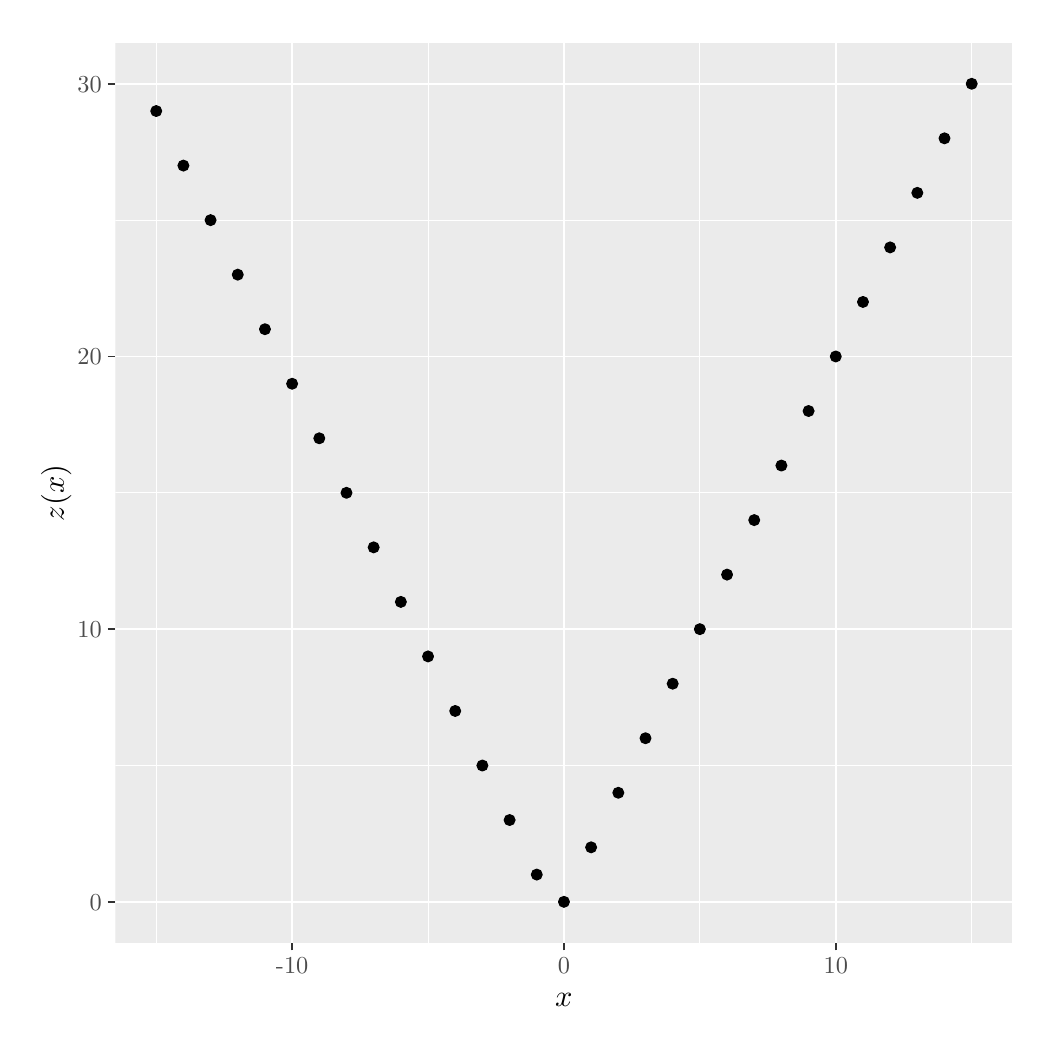
\begin{tikzpicture}[x=1pt,y=1pt]
\definecolor{fillColor}{RGB}{255,255,255}
\path[use as bounding box,fill=fillColor,fill opacity=0.00] (0,0) rectangle (361.35,361.35);
\begin{scope}
\path[clip] (  0.00,  0.00) rectangle (361.35,361.35);
\definecolor{drawColor}{RGB}{255,255,255}
\definecolor{fillColor}{RGB}{255,255,255}

\path[draw=drawColor,line width= 0.6pt,line join=round,line cap=round,fill=fillColor] (  0.00,  0.00) rectangle (361.35,361.35);
\end{scope}
\begin{scope}
\path[clip] ( 31.71, 30.69) rectangle (355.85,355.85);
\definecolor{fillColor}{gray}{0.92}

\path[fill=fillColor] ( 31.71, 30.69) rectangle (355.85,355.85);
\definecolor{drawColor}{RGB}{255,255,255}

\path[draw=drawColor,line width= 0.3pt,line join=round] ( 31.71, 94.73) --
	(355.85, 94.73);

\path[draw=drawColor,line width= 0.3pt,line join=round] ( 31.71,193.27) --
	(355.85,193.27);

\path[draw=drawColor,line width= 0.3pt,line join=round] ( 31.71,291.80) --
	(355.85,291.80);

\path[draw=drawColor,line width= 0.3pt,line join=round] ( 46.45, 30.69) --
	( 46.45,355.85);

\path[draw=drawColor,line width= 0.3pt,line join=round] (144.67, 30.69) --
	(144.67,355.85);

\path[draw=drawColor,line width= 0.3pt,line join=round] (242.89, 30.69) --
	(242.89,355.85);

\path[draw=drawColor,line width= 0.3pt,line join=round] (341.12, 30.69) --
	(341.12,355.85);

\path[draw=drawColor,line width= 0.6pt,line join=round] ( 31.71, 45.47) --
	(355.85, 45.47);

\path[draw=drawColor,line width= 0.6pt,line join=round] ( 31.71,144.00) --
	(355.85,144.00);

\path[draw=drawColor,line width= 0.6pt,line join=round] ( 31.71,242.54) --
	(355.85,242.54);

\path[draw=drawColor,line width= 0.6pt,line join=round] ( 31.71,341.07) --
	(355.85,341.07);

\path[draw=drawColor,line width= 0.6pt,line join=round] ( 95.56, 30.69) --
	( 95.56,355.85);

\path[draw=drawColor,line width= 0.6pt,line join=round] (193.78, 30.69) --
	(193.78,355.85);

\path[draw=drawColor,line width= 0.6pt,line join=round] (292.00, 30.69) --
	(292.00,355.85);
\definecolor{drawColor}{RGB}{0,0,0}
\definecolor{fillColor}{RGB}{0,0,0}

\path[draw=drawColor,line width= 0.4pt,line join=round,line cap=round,fill=fillColor] ( 46.45,331.22) circle (  1.96);

\path[draw=drawColor,line width= 0.4pt,line join=round,line cap=round,fill=fillColor] ( 56.27,311.51) circle (  1.96);

\path[draw=drawColor,line width= 0.4pt,line join=round,line cap=round,fill=fillColor] ( 66.09,291.80) circle (  1.96);

\path[draw=drawColor,line width= 0.4pt,line join=round,line cap=round,fill=fillColor] ( 75.91,272.10) circle (  1.96);

\path[draw=drawColor,line width= 0.4pt,line join=round,line cap=round,fill=fillColor] ( 85.74,252.39) circle (  1.96);

\path[draw=drawColor,line width= 0.4pt,line join=round,line cap=round,fill=fillColor] ( 95.56,232.68) circle (  1.96);

\path[draw=drawColor,line width= 0.4pt,line join=round,line cap=round,fill=fillColor] (105.38,212.97) circle (  1.96);

\path[draw=drawColor,line width= 0.4pt,line join=round,line cap=round,fill=fillColor] (115.20,193.27) circle (  1.96);

\path[draw=drawColor,line width= 0.4pt,line join=round,line cap=round,fill=fillColor] (125.02,173.56) circle (  1.96);

\path[draw=drawColor,line width= 0.4pt,line join=round,line cap=round,fill=fillColor] (134.85,153.85) circle (  1.96);

\path[draw=drawColor,line width= 0.4pt,line join=round,line cap=round,fill=fillColor] (144.67,134.15) circle (  1.96);

\path[draw=drawColor,line width= 0.4pt,line join=round,line cap=round,fill=fillColor] (154.49,114.44) circle (  1.96);

\path[draw=drawColor,line width= 0.4pt,line join=round,line cap=round,fill=fillColor] (164.31, 94.73) circle (  1.96);

\path[draw=drawColor,line width= 0.4pt,line join=round,line cap=round,fill=fillColor] (174.14, 75.03) circle (  1.96);

\path[draw=drawColor,line width= 0.4pt,line join=round,line cap=round,fill=fillColor] (183.96, 55.32) circle (  1.96);

\path[draw=drawColor,line width= 0.4pt,line join=round,line cap=round,fill=fillColor] (193.78, 45.47) circle (  1.96);

\path[draw=drawColor,line width= 0.4pt,line join=round,line cap=round,fill=fillColor] (203.60, 65.17) circle (  1.96);

\path[draw=drawColor,line width= 0.4pt,line join=round,line cap=round,fill=fillColor] (213.43, 84.88) circle (  1.96);

\path[draw=drawColor,line width= 0.4pt,line join=round,line cap=round,fill=fillColor] (223.25,104.59) circle (  1.96);

\path[draw=drawColor,line width= 0.4pt,line join=round,line cap=round,fill=fillColor] (233.07,124.29) circle (  1.96);

\path[draw=drawColor,line width= 0.4pt,line join=round,line cap=round,fill=fillColor] (242.89,144.00) circle (  1.96);

\path[draw=drawColor,line width= 0.4pt,line join=round,line cap=round,fill=fillColor] (252.72,163.71) circle (  1.96);

\path[draw=drawColor,line width= 0.4pt,line join=round,line cap=round,fill=fillColor] (262.54,183.41) circle (  1.96);

\path[draw=drawColor,line width= 0.4pt,line join=round,line cap=round,fill=fillColor] (272.36,203.12) circle (  1.96);

\path[draw=drawColor,line width= 0.4pt,line join=round,line cap=round,fill=fillColor] (282.18,222.83) circle (  1.96);

\path[draw=drawColor,line width= 0.4pt,line join=round,line cap=round,fill=fillColor] (292.00,242.54) circle (  1.96);

\path[draw=drawColor,line width= 0.4pt,line join=round,line cap=round,fill=fillColor] (301.83,262.24) circle (  1.96);

\path[draw=drawColor,line width= 0.4pt,line join=round,line cap=round,fill=fillColor] (311.65,281.95) circle (  1.96);

\path[draw=drawColor,line width= 0.4pt,line join=round,line cap=round,fill=fillColor] (321.47,301.66) circle (  1.96);

\path[draw=drawColor,line width= 0.4pt,line join=round,line cap=round,fill=fillColor] (331.29,321.36) circle (  1.96);

\path[draw=drawColor,line width= 0.4pt,line join=round,line cap=round,fill=fillColor] (341.12,341.07) circle (  1.96);
\end{scope}
\begin{scope}
\path[clip] (  0.00,  0.00) rectangle (361.35,361.35);
\definecolor{drawColor}{gray}{0.30}

\node[text=drawColor,anchor=base east,inner sep=0pt, outer sep=0pt, scale=  0.88] at ( 26.76, 42.44) {0};

\node[text=drawColor,anchor=base east,inner sep=0pt, outer sep=0pt, scale=  0.88] at ( 26.76,140.97) {10};

\node[text=drawColor,anchor=base east,inner sep=0pt, outer sep=0pt, scale=  0.88] at ( 26.76,239.50) {20};

\node[text=drawColor,anchor=base east,inner sep=0pt, outer sep=0pt, scale=  0.88] at ( 26.76,338.04) {30};
\end{scope}
\begin{scope}
\path[clip] (  0.00,  0.00) rectangle (361.35,361.35);
\definecolor{drawColor}{gray}{0.20}

\path[draw=drawColor,line width= 0.6pt,line join=round] ( 28.96, 45.47) --
	( 31.71, 45.47);

\path[draw=drawColor,line width= 0.6pt,line join=round] ( 28.96,144.00) --
	( 31.71,144.00);

\path[draw=drawColor,line width= 0.6pt,line join=round] ( 28.96,242.54) --
	( 31.71,242.54);

\path[draw=drawColor,line width= 0.6pt,line join=round] ( 28.96,341.07) --
	( 31.71,341.07);
\end{scope}
\begin{scope}
\path[clip] (  0.00,  0.00) rectangle (361.35,361.35);
\definecolor{drawColor}{gray}{0.20}

\path[draw=drawColor,line width= 0.6pt,line join=round] ( 95.56, 27.94) --
	( 95.56, 30.69);

\path[draw=drawColor,line width= 0.6pt,line join=round] (193.78, 27.94) --
	(193.78, 30.69);

\path[draw=drawColor,line width= 0.6pt,line join=round] (292.00, 27.94) --
	(292.00, 30.69);
\end{scope}
\begin{scope}
\path[clip] (  0.00,  0.00) rectangle (361.35,361.35);
\definecolor{drawColor}{gray}{0.30}

\node[text=drawColor,anchor=base,inner sep=0pt, outer sep=0pt, scale=  0.88] at ( 95.56, 19.68) {-10};

\node[text=drawColor,anchor=base,inner sep=0pt, outer sep=0pt, scale=  0.88] at (193.78, 19.68) {0};

\node[text=drawColor,anchor=base,inner sep=0pt, outer sep=0pt, scale=  0.88] at (292.00, 19.68) {10};
\end{scope}
\begin{scope}
\path[clip] (  0.00,  0.00) rectangle (361.35,361.35);
\definecolor{drawColor}{RGB}{0,0,0}

\node[text=drawColor,anchor=base,inner sep=0pt, outer sep=0pt, scale=  1.10] at (193.78,  7.64) {$x$};
\end{scope}
\begin{scope}
\path[clip] (  0.00,  0.00) rectangle (361.35,361.35);
\definecolor{drawColor}{RGB}{0,0,0}

\node[text=drawColor,rotate= 90.00,anchor=base,inner sep=0pt, outer sep=0pt, scale=  1.10] at ( 13.08,193.27) {$z(x)$};
\end{scope}
\end{tikzpicture}

\caption{\label{fig:zigzag}The zig-zag encoding applied to integers -15 to 15. As we can see, it is similar to the absolute value function but is doubled and shifted on the negative $x$-axis to ensure injectivity.}
\end{figure}


Altogether, the state-of-the-art compression method first applies differential
coding followed by zig-zag encoding to obtain the `zig-zag deltas' of the data.
Then, svb is applied to the zig-zag deltas followed by the zstd algorithm. ONT
believe that using svb16 instead of svb here achieves better compression, but the
benchmark results presented in Chapter \ref{chap:results} reveal otherwise.
Hence, zstd-svb-zd is the current state-of-the-art approach for losslessly
compressing nanopore signal data.

zstd-svb-zd is fast in practice for both compression and decompression. This is
mostly because its sub-methods (zstd and svb) have been highly optimised.
Furthermore, it only requires at least four passes of the data during
compression; finding the zig-zag deltas takes two, svb takes one and zstd
requires at least one. The same is true for decompression. However, the method
is very generic, only using the fact that the signal's deltas are small to
achieve better compression. Hence, by analysing the data and understanding its
characteristics, we should be able to save more space.

This leads us to the following chapter, where we will conduct a systematic
analysis of the data, its characteristics and transformations.
